\pagenumbering{arabic}
%\documentclass[slides]{beamer}
\documentclass[mathserif, 8pt]{beamer}
\usepackage[framesassubsections]{beamerprosper}
\setbeamercovered{transparent}
%\documentclass[slides,hyperref={pdfpagelabels=false}]{beamer}
%\documentclass[handout,gray]{beamer}
\usepackage[T1]{fontenc}
\usepackage[utf8]{inputenc}
\usepackage{textcomp}
\usepackage{algorithm}
\usepackage{algorithmic}
\usepackage{color}
\usepackage{verbatim}
\usepackage{amsbsy}
\usepackage{multirow}
\usepackage{multicol}
\usepackage{booktabs} % Make some nice tables
\usepackage{ae,aecompl}

%%%%%%%%%%%% COULEURS %%%%%%%%%%%%%%%%%%%%%%%%%%%

\mode<presentation>
{
  \definecolor{beamerstructure}{RGB}{43,79,112}
  \definecolor{sidebackground}{RGB}{230,242,250}
  \definecolor{CTCC}{RGB}{133,188,228}
  \color{beamerstructure}
  \usetheme{default}
  \usepackage{courier}
  \beamertemplateballitem
\setbeamertemplate{navigation symbols}{}
%\setbeamertemplate{sidebar left}{\thispdfpagelabel{\insertframenumber}}
%\setbeamertemplate{footline}{\quad\insertframenumber}
%\usecolortheme{CTCC}
}
\usebackgroundtemplate{\includegraphics[width=1.02\paperwidth]
{../templets/ctcc_general.jpg}}

\title{\\\vspace{1cm}
MRGrid}
\subtitle{{Accurate and reliable DFT grids using multiwavelets}}
\author{Stig Rune Jensen}
\institute[CTCC]{\\[-6mm]stig.r.jensen@uit.no\\
[6mm]UiT - The Arctic University of Norway\\[6mm]
\includegraphics[height=1.5cm]{../templets/uio.pdf}\hspace{1cm} 
\includegraphics[height=1.5cm]{../templets/sff.pdf}\hspace{1cm}
\includegraphics[height=1.5cm]{../templets/uit.pdf}}
\date{January 30, 2015}

\newcommand{\gb}[1]{green!#1!black}
\newcommand{\rb}[1]{red!#1!black}
\newcommand{\bb}[1]{blue!#1!black}
\newcommand{\coleq}{red!60!black}
\newcommand{\du}{\textrm{d}}

\newcommand{\mydef}{\stackrel{\text{def}}{\hbox{=}}} 
\newcommand{\Node}{\texttt{Node\ }}
\newcommand{\node}{\texttt{node\ }}
\newcommand{\nodes}{\texttt{nodes\ }}
\newcommand{\Tree}{\texttt{Tree\ }}
\newcommand{\tree}{\texttt{tree\ }}
\newcommand{\trees}{\texttt{trees\ }}

\begin{document}

\footnotesize
\setlength{\unitlength}{\textwidth}

{
\usebackgroundtemplate{\includegraphics[width=1.02\paperwidth]
{../templets/ctcc_forside.jpg}}
\maketitle
}

\begin{frame}
    \frametitle{Traditional grids}
    \begin{columns}
    \begin{column}{0.6\linewidth}
    \centering

    \vspace{10mm}

    \begin{itemize}
        \item Spherical grids
        \item Good accuracy with \textbf{few} grid points
        \item Based on atomic symmetry
        \item Fitted to important properties like total energy and geometry
        \item Possibly less accurate for higher order properties
        \item Decomposed into atomic contributions
    \end{itemize}

    \vspace{2mm}

    \begin{equation}
        \nonumber
        \int F(r) dr \approx \sum_K^{atoms} \sum_i^{grid} \omega_K(r_i) F(r_i)
    \end{equation}

    \vspace{15mm}

    \scriptsize
    A. D. Becke, 
    {\it JCP}, \textbf{88} (4), 1988\\
    O. Treutler, R. Ahlrichs,
    {\it JCP}, \textbf{102} (1), 1995\\
    R. E. Stratman {\it et. al.}
    {\it Chem. Phys. Lett.}, \textbf{257}, 1996
    
    \end{column}

    \begin{column}{0.4\linewidth}
    \centering
    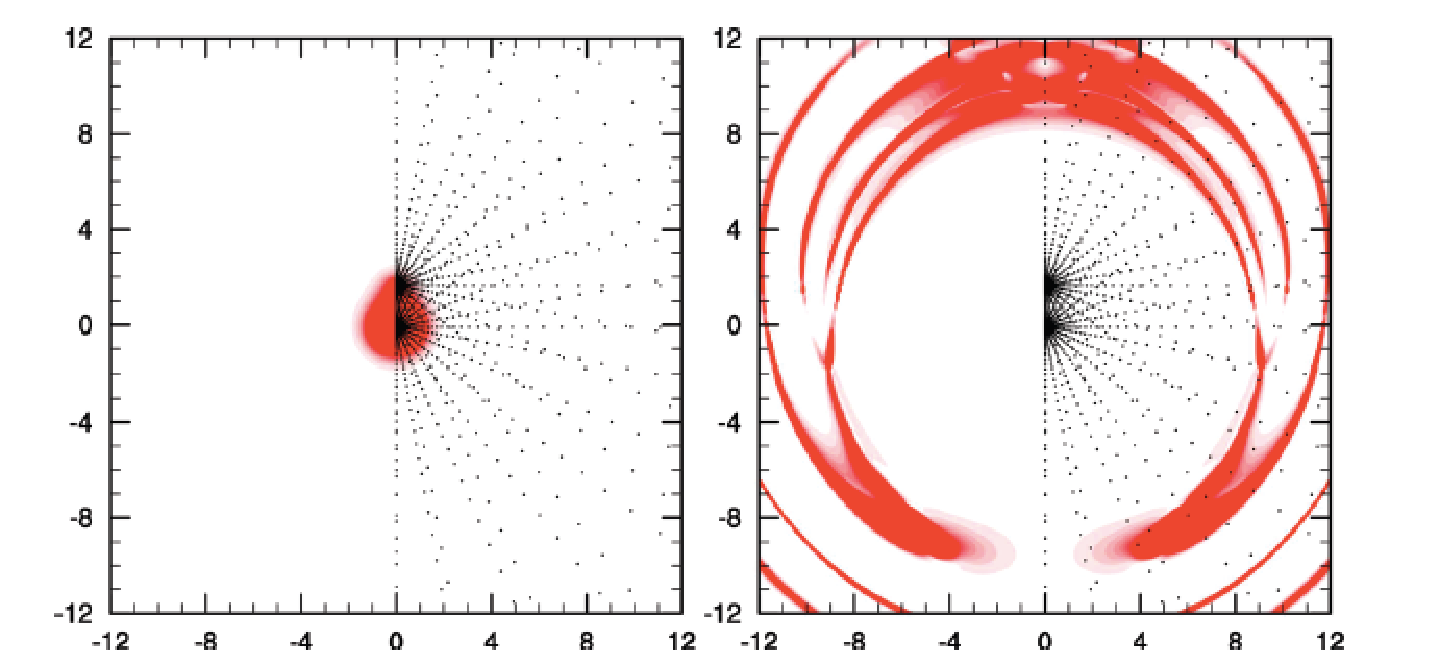
\includegraphics[clip, viewport = 0 0 650 350, angle=-90, scale=0.3]{figures/radialgrid.pdf}

    \vspace {2mm}

    \scriptsize
    U. Ekstr\"{o}m, {\it et. al.}
    {\it JCTC}, \textbf{6} (7), 2010
    \end{column}
    \end{columns}
\end{frame}

\begin{frame}
    \frametitle{MultiResolution Grids}
    \begin{columns}
    \begin{column}{0.5\linewidth}
    \begin{itemize}
        \item Cartesian grids
        \item Not constructed for specific properties
        \item Guaranteed accuracy with \textbf{many} grid points
        \item Can be individually fitted to each function
        \item Decomposed into cubic cells
    \end{itemize}

    \vspace{5mm}

    \begin{equation}
        \nonumber
        \int F(r) dr \approx \sum_K^{cells} \sum_i^{grid} \omega_K(r_i) F(r_i)
    \end{equation}
    \end{column}

    \begin{column}{0.5\linewidth}
    \centering
    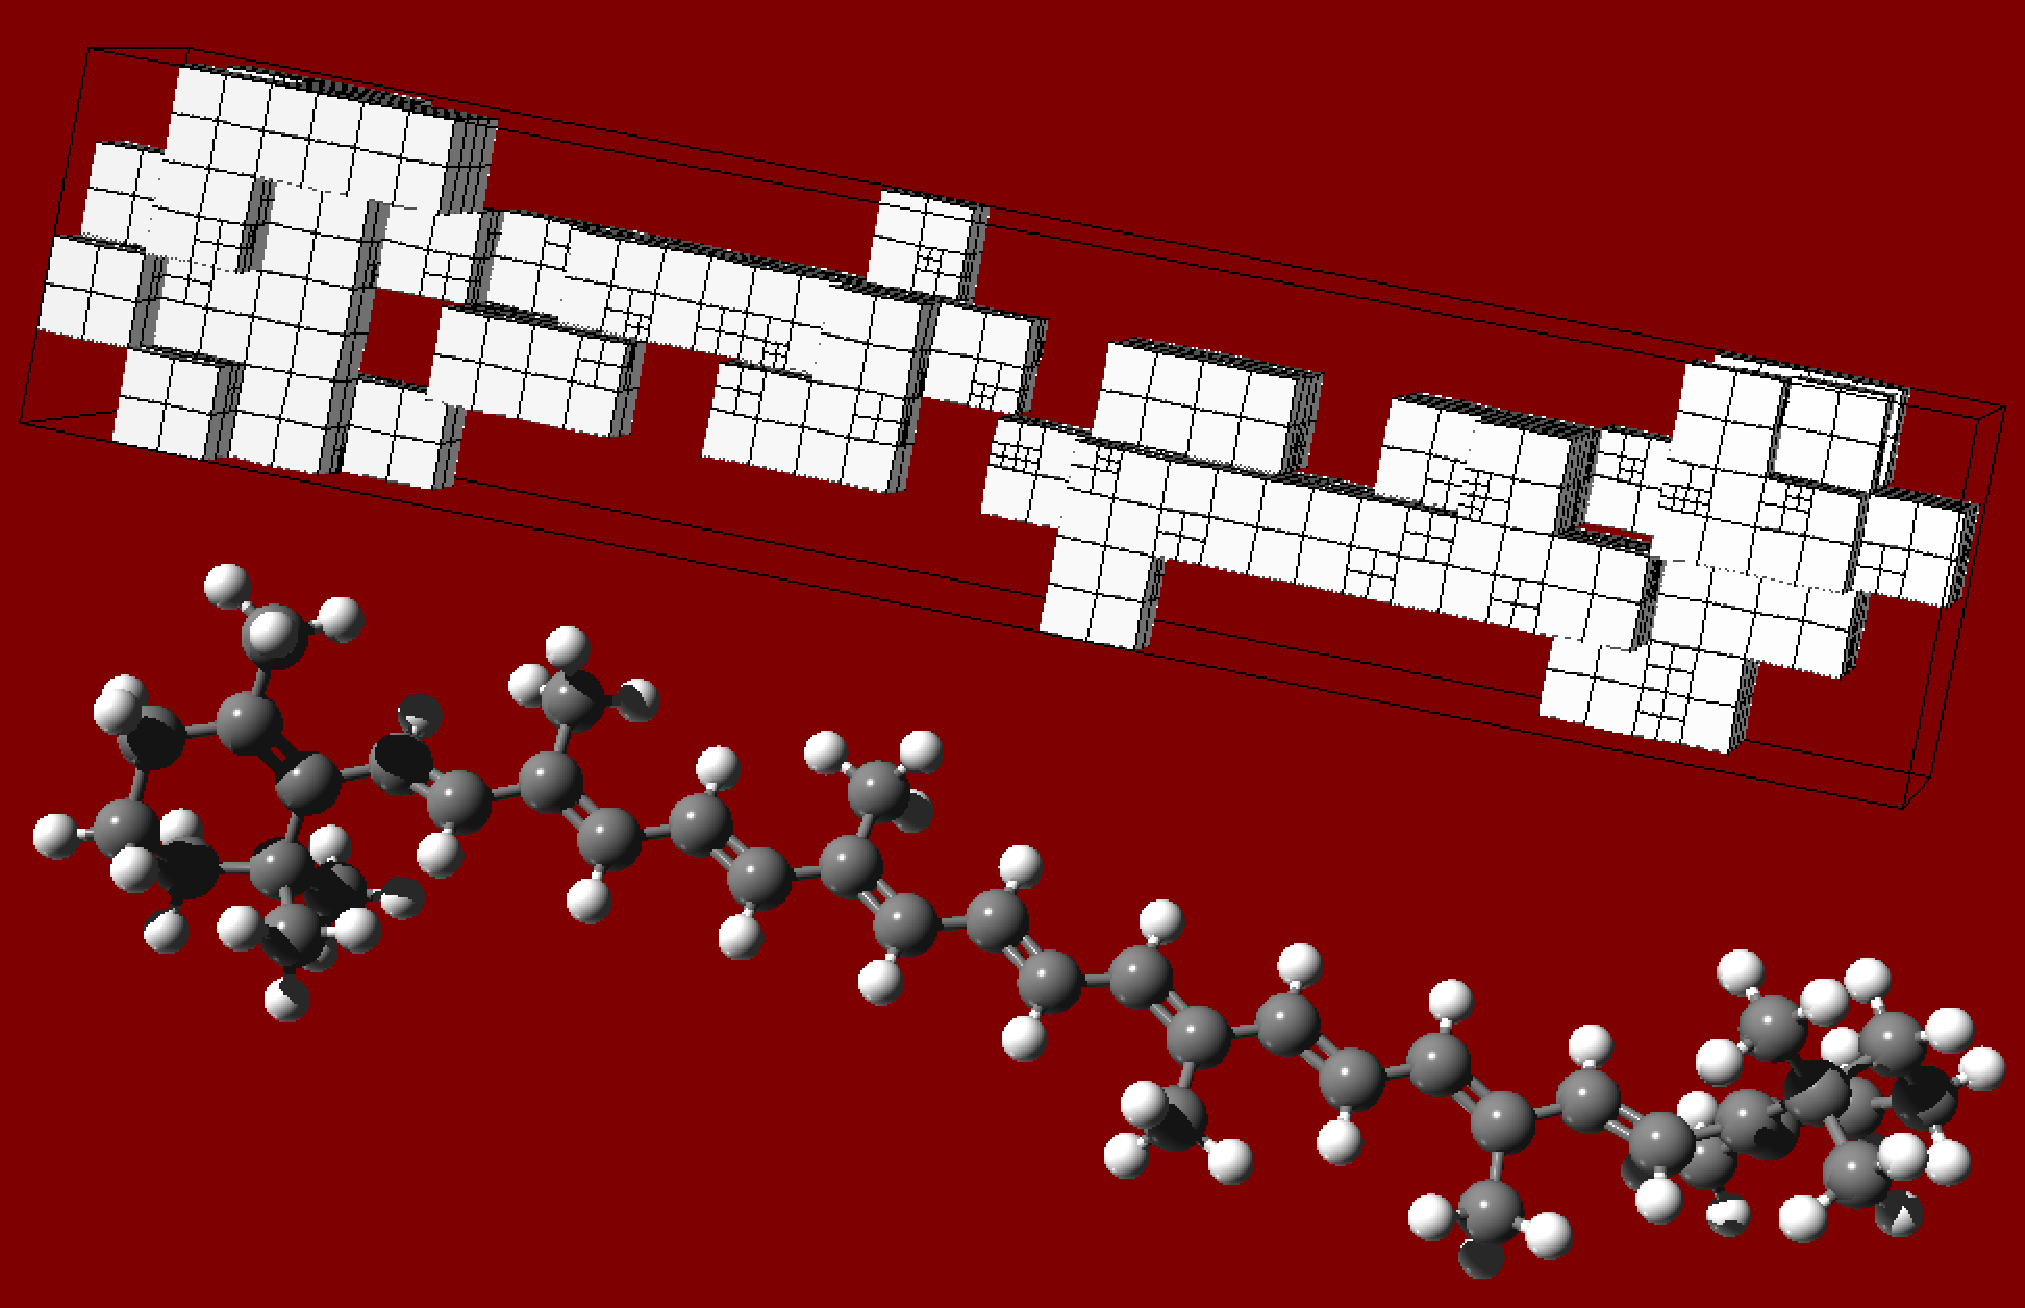
\includegraphics[angle=-90, scale=0.2]{figures/caroteneGrid.pdf}
    \end{column}
    \end{columns}
\end{frame}


\begin{frame}
\frametitle{Multiwavelets}
\begin{columns}

\begin{column}[b]{0.55\linewidth}
\begin{itemize}
    \item   \textbf{Scaling functions} are polynomials or order $\leq k$\\
	    on the unit interval
    \item   \textbf{Dilation and translation} to refinement scale $n$
	    \begin{equation}
		\nonumber
		\phi_l^n(x) = 2^{n/2}\phi(2^nx-l)
	    \end{equation}
    \item   At scale $n$ there are $2^n$ subintervals
    \item   The length of each subinterval is $2^{-n}$
    \item   \textbf{Scaling projection} at scale $N$
	    \begin{equation}
		\nonumber
		f(x) \approx f^N(x) = \sum_l s_l^N \phi_l^N(x)
	    \end{equation}
	    \ \\
	    \ \\
    \item   For a $k$-order basis in $d$ dimensions there are\\
	    $\left(2(k+1)\right)^{nd}$ basis functions at scale $n$\\
\end{itemize}
\centering
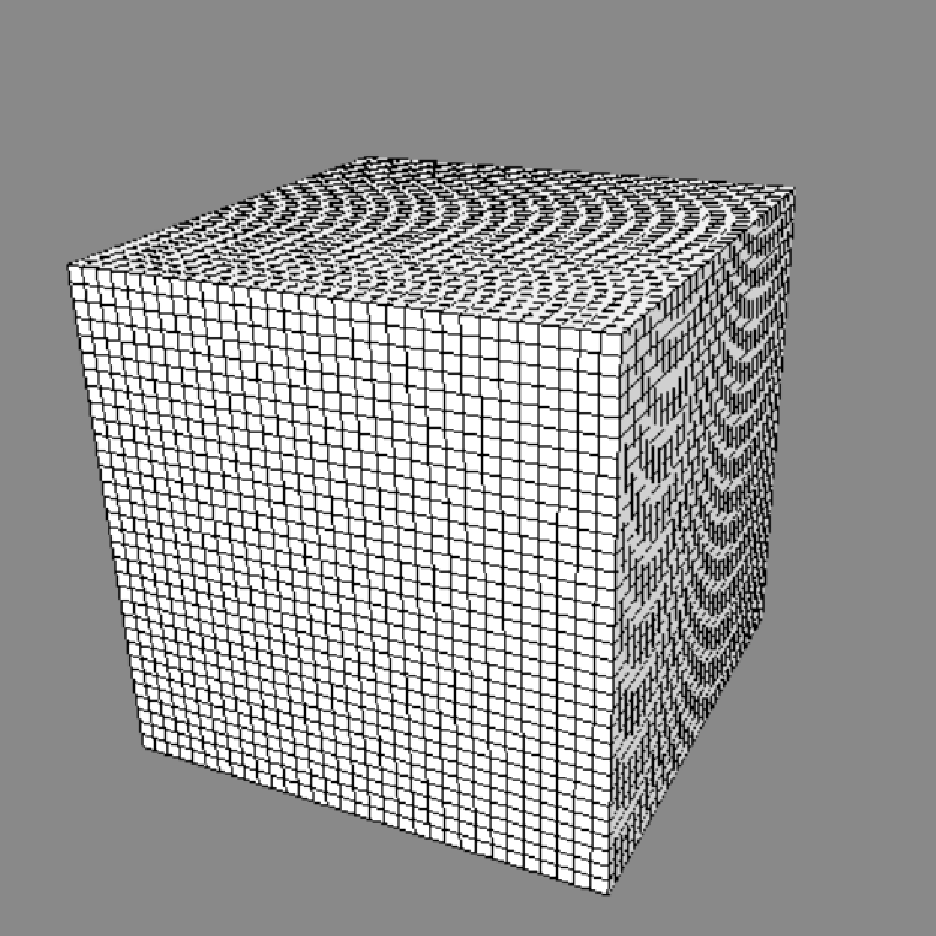
\includegraphics[scale=0.2]{figures/unifgrid.pdf}
\end{column}

\begin{column}[b]{0.45\linewidth}
\centering
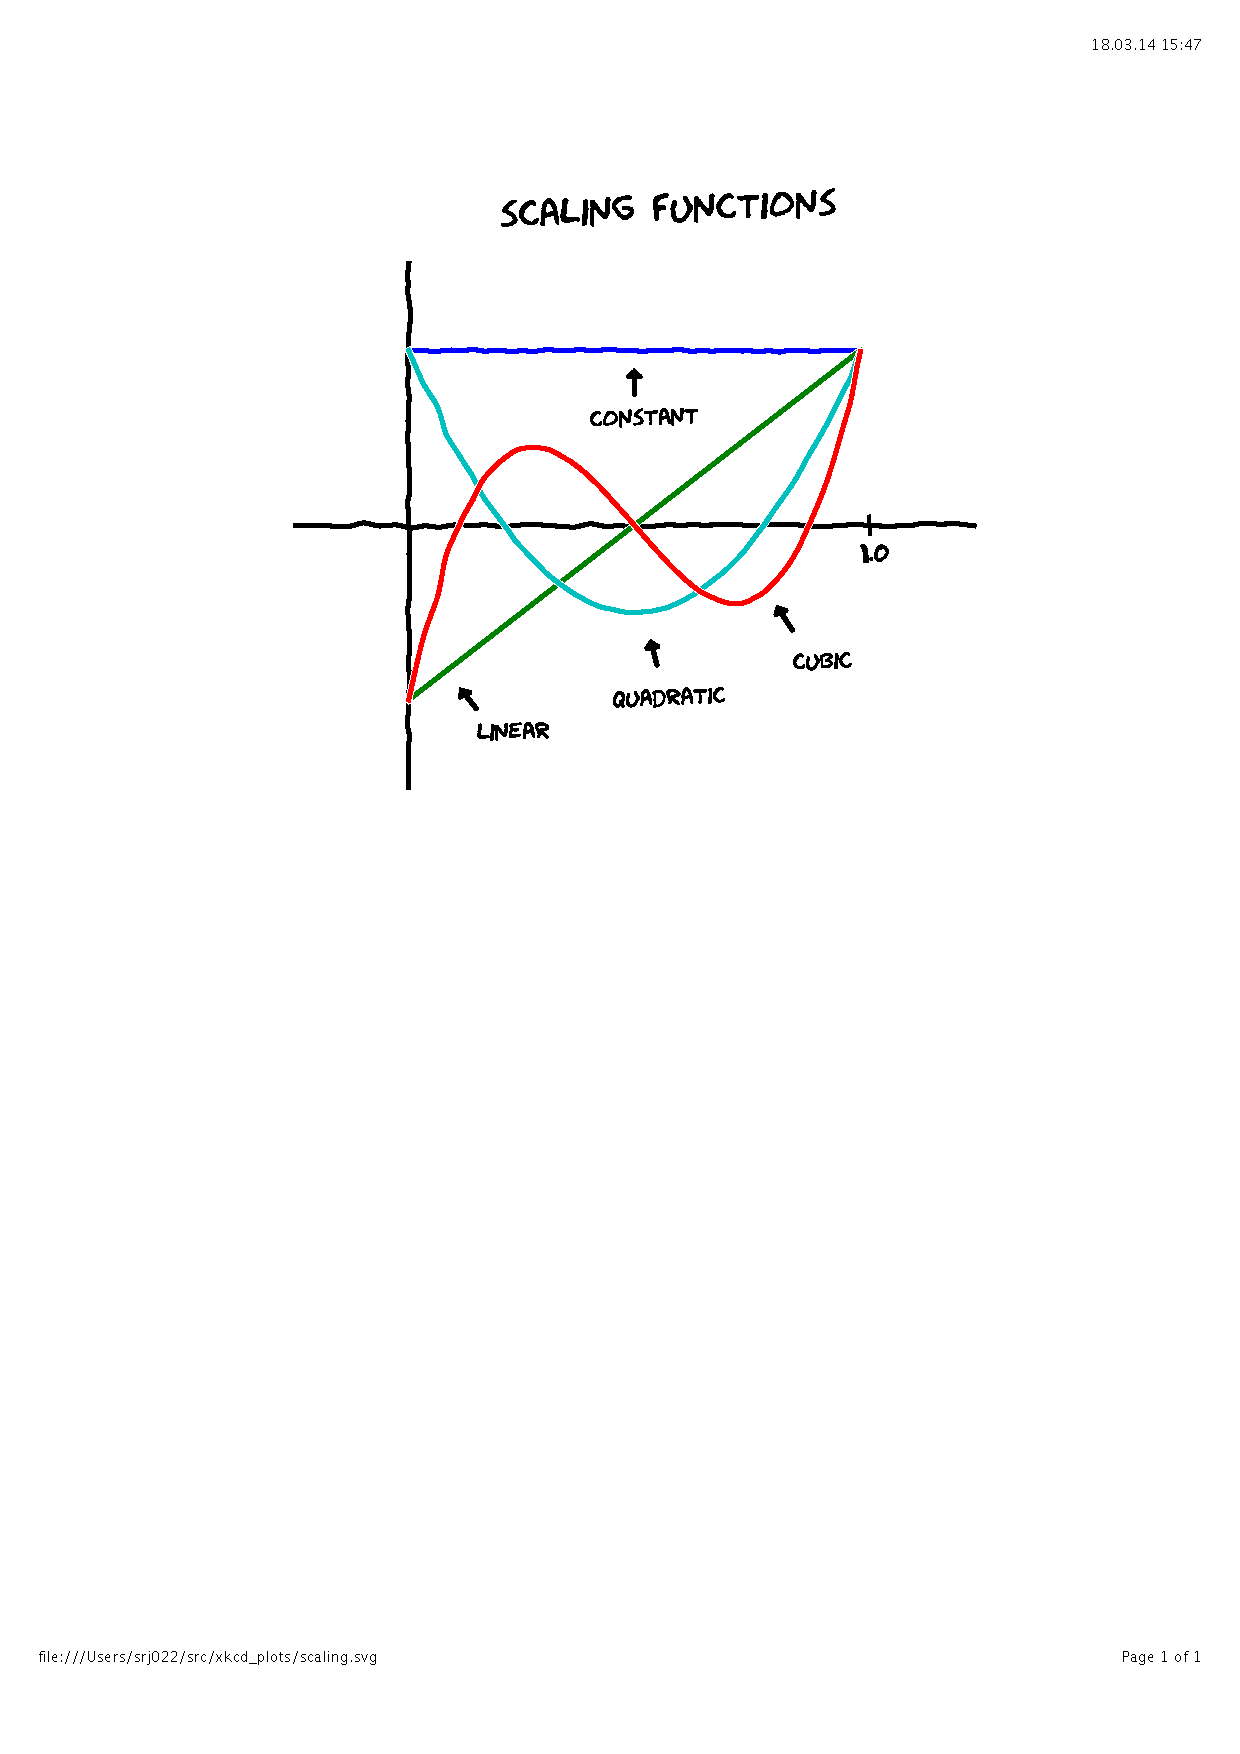
\includegraphics[scale=0.3, clip, viewport=150 450 450 750]
    {figures/scaling.pdf}\\
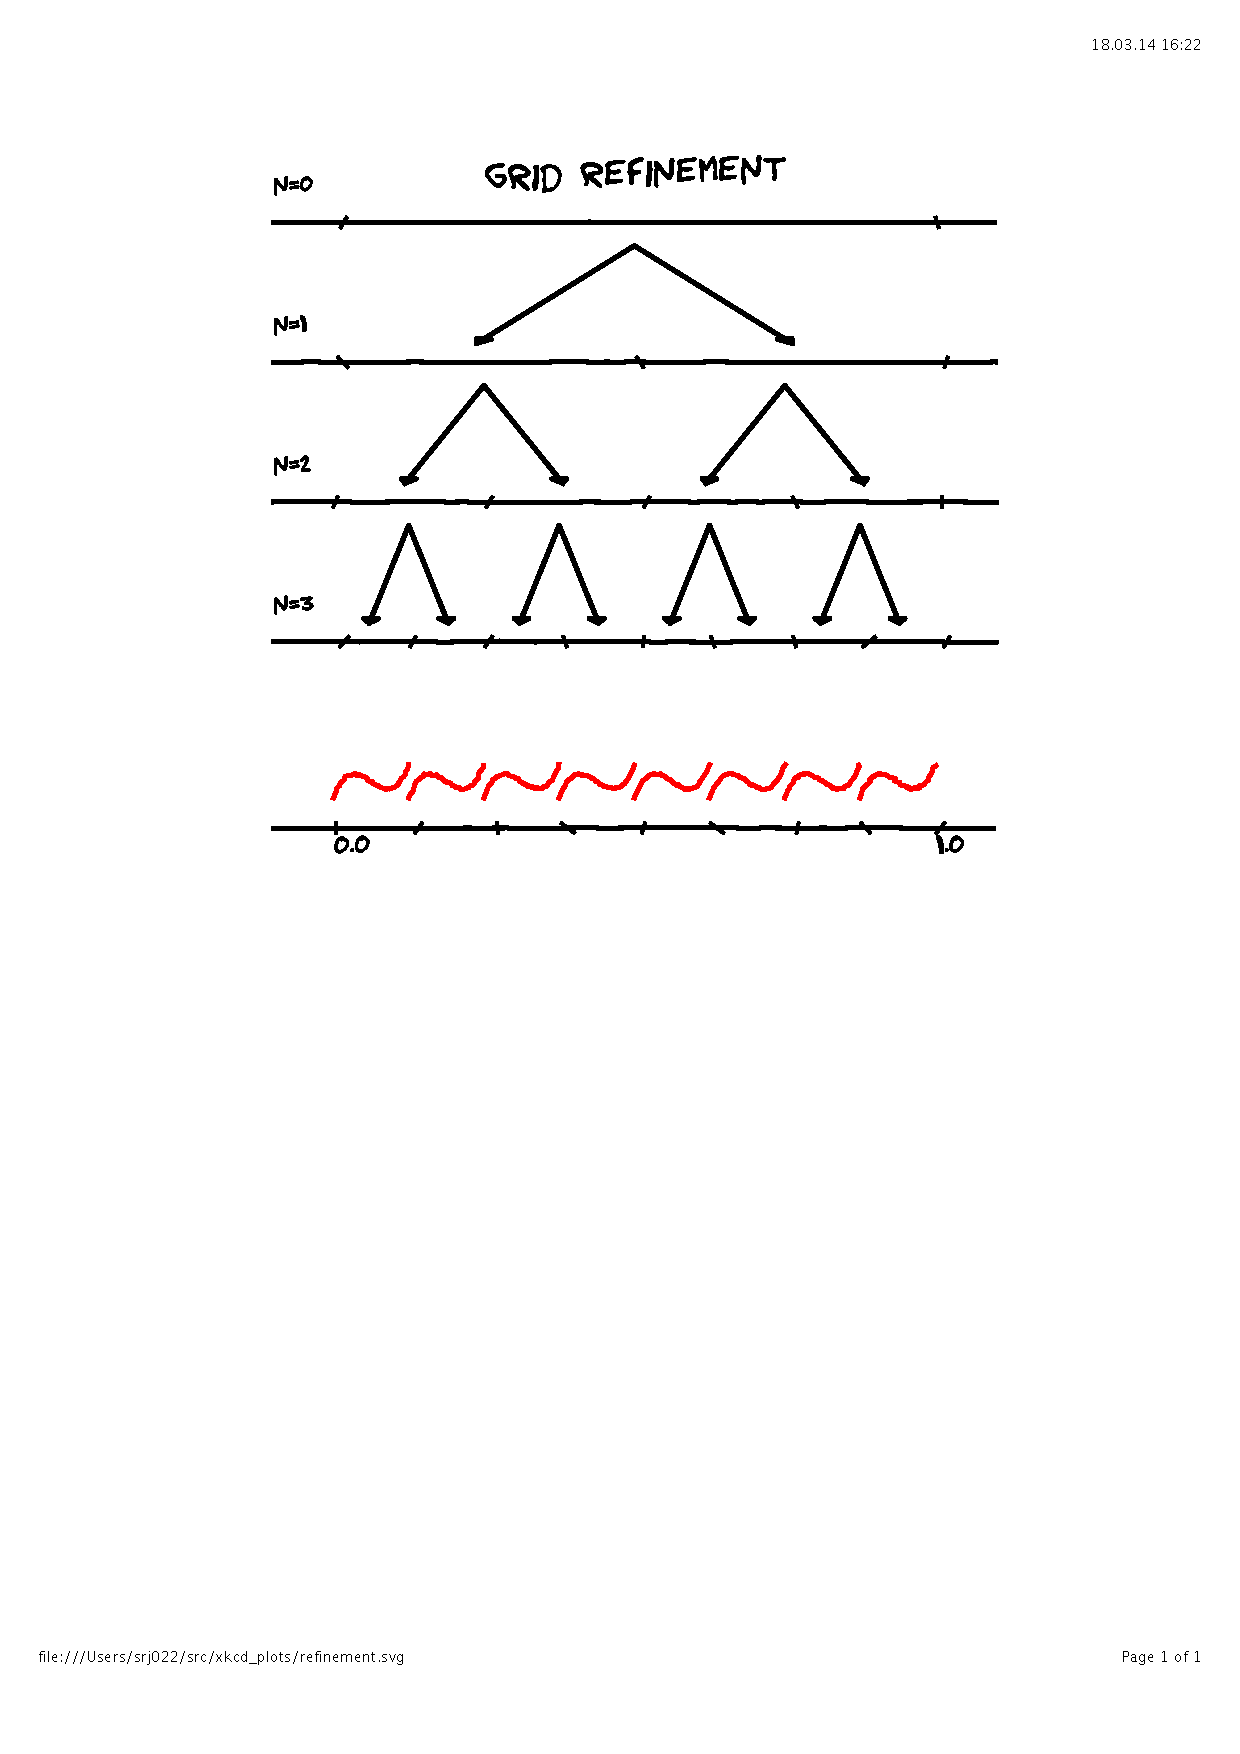
\includegraphics[scale=0.3, clip, viewport=100 400 500 800]
    {figures/refinement.pdf}
\end{column}

\end{columns}
\end{frame}


%\begin{frame}
%\frametitle{Multiwavelets}
%\centering
%\only<1>{\ \ \ \includegraphics[clip, viewport=50 100 600 800, scale=0.5]
%    {figures/f0.pdf}}
%\only<2>{\ \ \includegraphics[clip, viewport=50 100 600 800, scale=0.5]
%    {figures/f1.pdf}}
%\only<3>{\ \includegraphics[clip, viewport=50 100 600 800, scale=0.5]
%    {figures/f2.pdf}}
%\only<4>{\includegraphics[clip, viewport=50 100 600 800, scale=0.5]
%    {figures/f3.pdf}}
%\only<5>{\includegraphics[clip, viewport=50 100 600 800, scale=0.5]
%    {figures/f4.pdf}}
%\end{frame}


\begin{frame}
\frametitle{Multiwavelets}
\begin{columns}

\begin{column}[b]{0.55\linewidth}
\begin{itemize}
    \item   \textbf{Wavelet functions} are piecewise polynomials
    \item   \textbf{Wavelet projection} at scale $N$
	\begin{equation}
	    \nonumber
	    df^n(x) = f^{n+1}(x) - f^{n}(x)
	\end{equation}
	\ \\
    \item   Alternative \textbf{multiresolution} representation
	\begin{equation}
	    \nonumber
	    f^N(x) = f^{0}(x) + \sum_{n=0}^{N-1} df^{n}(x)
	\end{equation}
    \item   Allows for \textbf{adaptive refinement} by local thresholding
	\begin{equation}
	    \nonumber
	    \|df_l^n\| < \frac{\epsilon}{2^{n/2}}\|f\|
	\end{equation}
    \item   Representations with \textbf{guaranteed precision} $\epsilon$
\end{itemize}
\ \\
\ \\
\end{column}

\begin{column}[b]{0.45\linewidth}
\centering
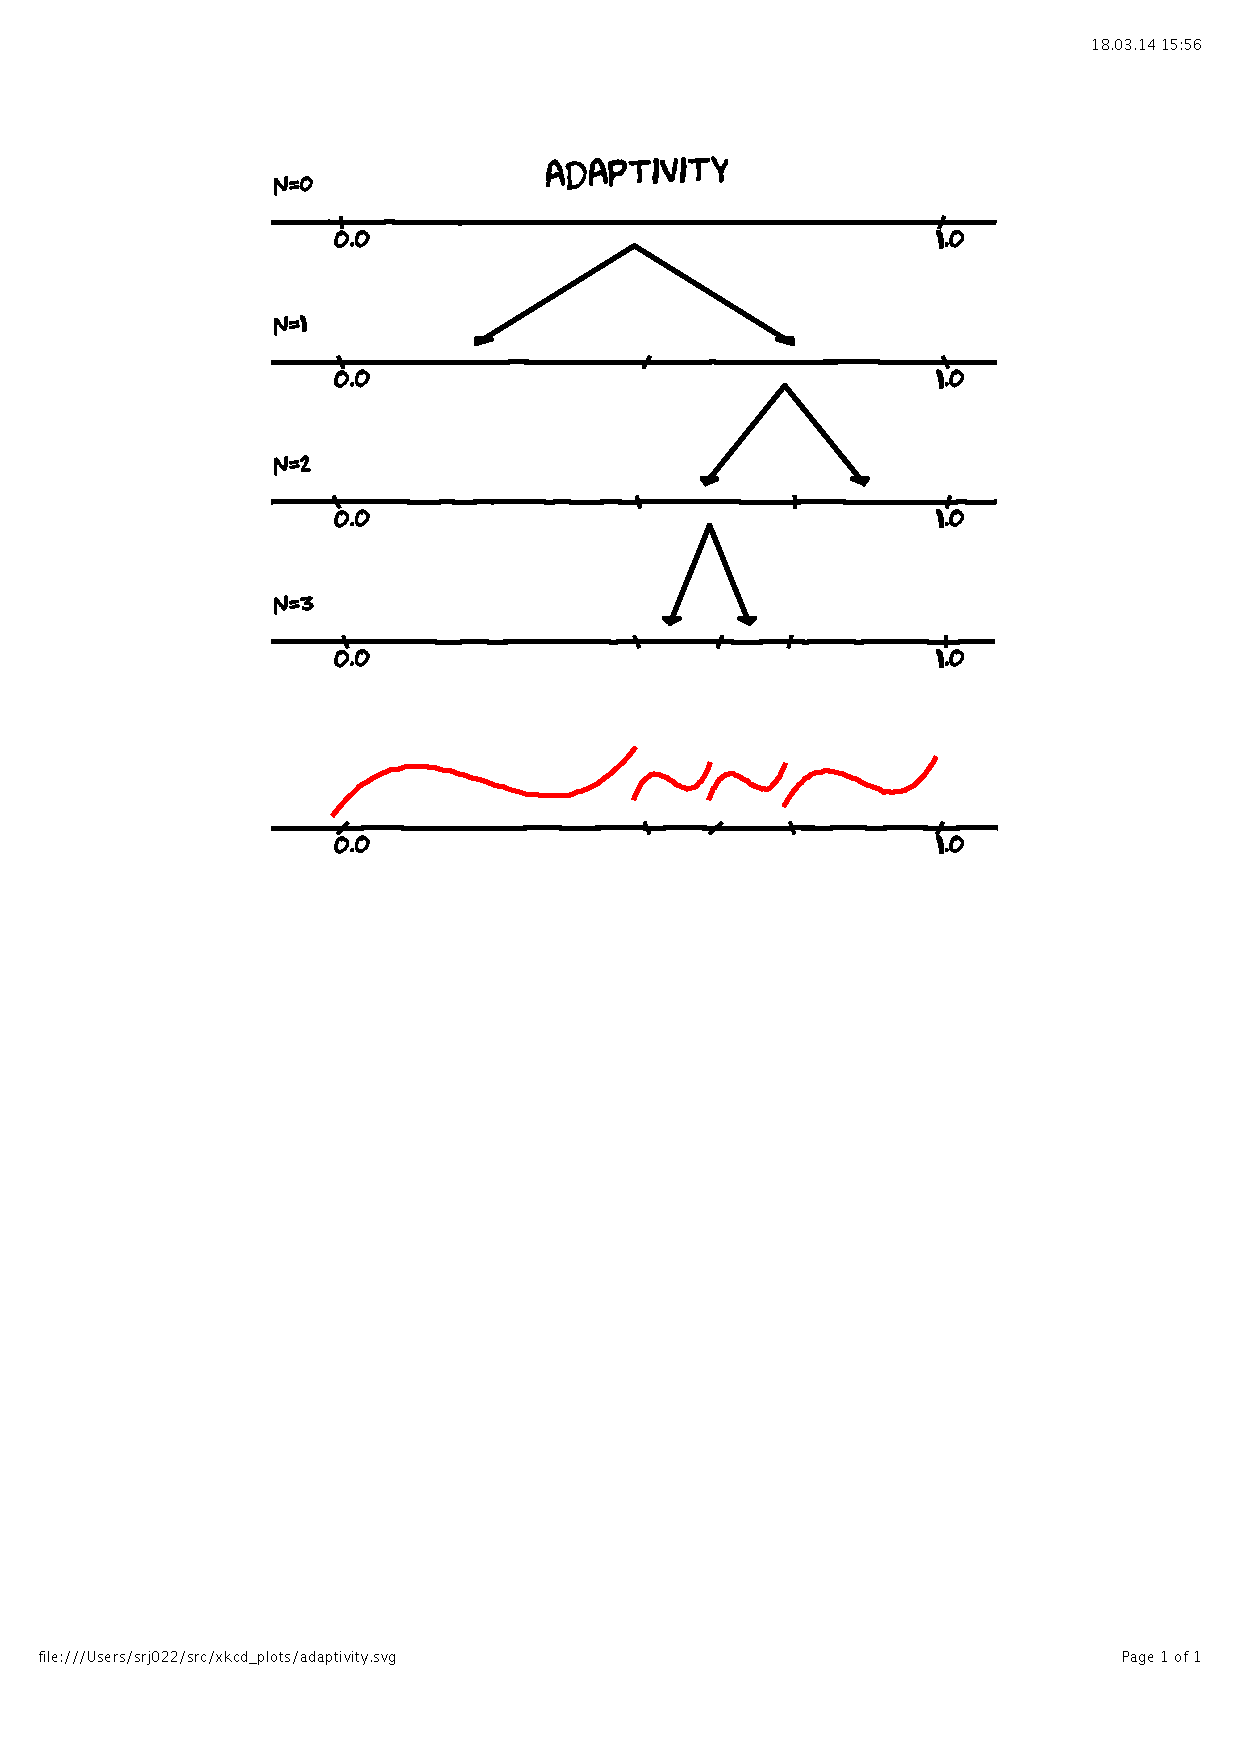
\includegraphics[scale=0.3, clip, viewport=100 400 500 800]
    {figures/adaptivity.pdf}
\end{column}

\end{columns}
\ \\
\centering
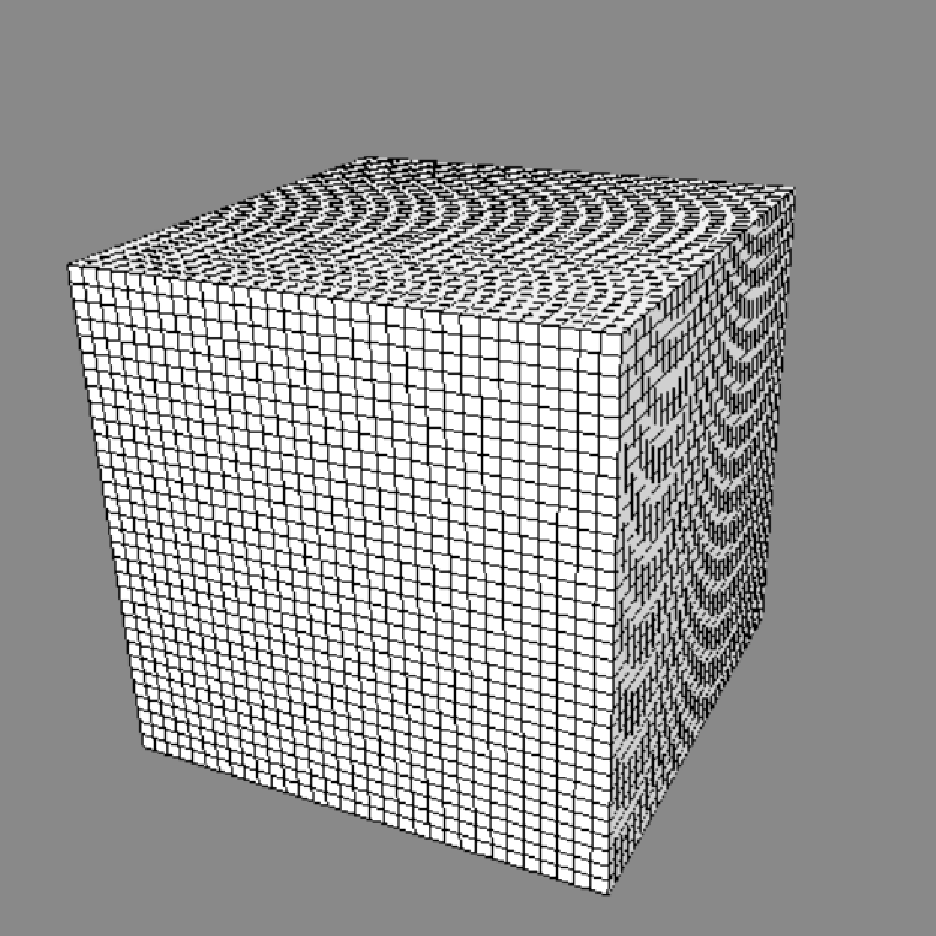
\includegraphics[scale=0.2]{figures/unifgrid.pdf}
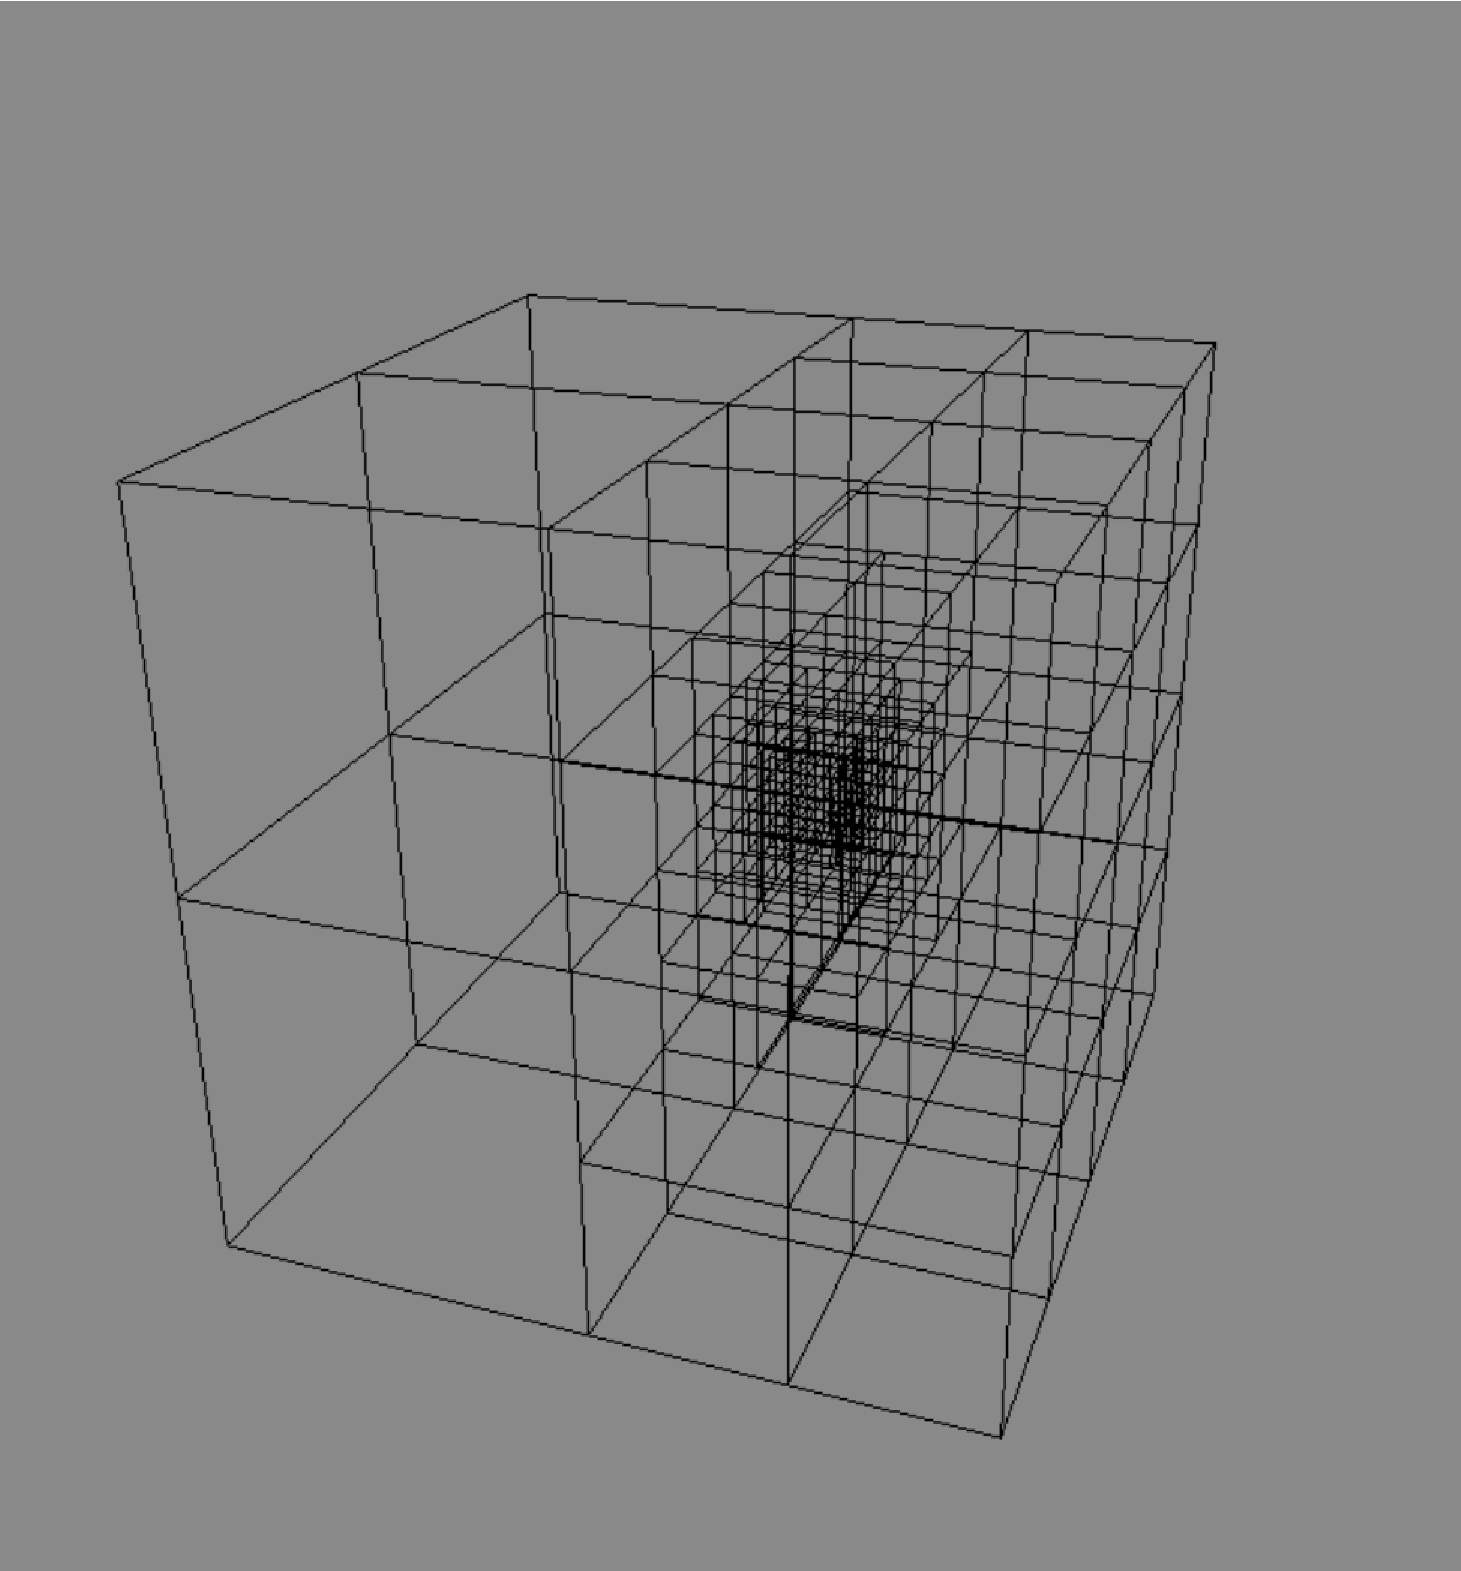
\includegraphics[scale=0.1192]{figures/adapgrid.pdf}
\end{frame}

\begin{frame}
    \frametitle{MRCPP features}
    \begin{itemize}
        \item Currently: precision based
        \item All grids are function specific
        \item On the fly adaptivity
        \item Complicated algorithms
        \item Difficult to load balance
    \end{itemize}
    \vspace{5mm}
    \begin{itemize}
        \item Future: grid based
        \item Fixed grids in each SCF iteration
        \item Grid refinement between iterations
        \item Fixed grids $\longrightarrow$ better performance
        \item Better error control for \emph{local} operators
    \end{itemize}
\end{frame}

\begin{frame}
    \frametitle{Local operators}
    \begin{columns}
    \begin{column}{0.3\linewidth}
    \normalsize
    \centering
    \begin{equation}
        \nonumber
        \rho \longrightarrow \nabla \rho
    \end{equation}
    
    \vspace{3mm}

    \begin{equation}
        \nonumber
        \rho \longrightarrow E_{xc}
    \end{equation}
    
    \vspace{2mm}

    \begin{equation}
        \nonumber
        \rho \longrightarrow \frac{\delta E_{xc}}{\delta \rho}
    \end{equation}
    
    \vspace{1mm}

    \begin{equation}
        \nonumber
        \rho \longrightarrow \frac{\delta^2 E_{xc}}{\delta \rho^2}
    \end{equation}
    
    \vspace{5mm}

    \end{column}
    \begin{column}{0.7\linewidth}
    \centering

    Treutler and Ahlrichs claim that the error $\Delta E_{xc}$ in the XC 
    energy\\ is related to the error $\Delta N$ in the charge integral

    \vspace{3mm}

    \begin{equation}
        \nonumber
        |\Delta E_{xc}| \leq\Delta N
    \end{equation}

    \vspace{5mm}

    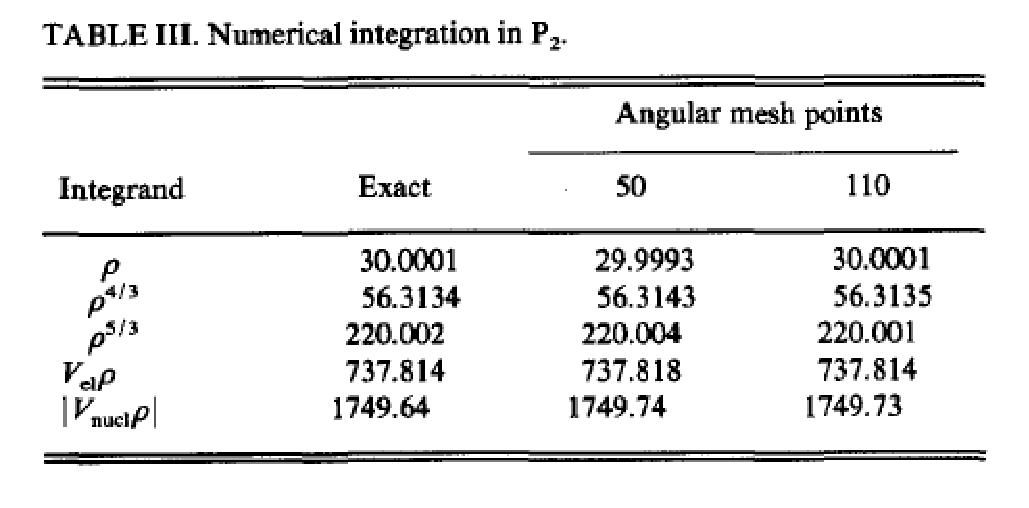
\includegraphics[scale = 0.4]{figures/beckeAccuracy.pdf}

    \vspace{1mm}

    \scriptsize
    A. D. Becke, 
    {\it JCP}, \textbf{88} (4), 1988

    \end{column}
    \end{columns}
\end{frame}

\begin{frame}
    \frametitle{MRGrid features}
    \hspace{45mm} \textbf{Basic}
    \begin{columns}
    \begin{column}{0.3\linewidth}
    \end{column}
    \begin{column}{0.5\linewidth}
    \begin{itemize}
        \item generateGrid(molecule)
        \item getQuadraturePoints()
        \item getQuadratureValues()
        \item getQuadratureWeights()
    \end{itemize}
    \end{column}
    \begin{column}{0.2\linewidth}
    \end{column}
    \end{columns}

    \vspace{15mm}

    \begin{columns}
    \begin{column}{0.1\linewidth}
    \end{column}
    \begin{column}{0.4\linewidth}
    \hspace{5mm} \textbf{More advanced}
    \begin{itemize}
        \item project(function)
        \item estimateError()
        \item refineGrid(prec)
        \item integrate()
        \item innerProduct()
        \item arithmetic operations
        \item Coulomb operator
    \end{itemize}
    \end{column}
    \begin{column}{0.5\linewidth}
    \hspace{5mm} \textbf{Algorithm}
    \begin{itemize}
        \item Generate initial grid
        \item \textbf{Start SCF cycle}
        \item Project density
        \item Compute potentials
        \item Estimate errors
        \item \textbf{Finish SCF cycle}
        \item Refine grids if necessary
    \end{itemize}
    \end{column}
    \end{columns}
\end{frame}


\begin{frame}
\frametitle{Grid adaptation}
\centering

\textbf{Grid adaptation $10^{-3}$ based ONLY on input density $CH_4$}
\begin{table}
\centering
\begin{tabular}{r|rrr|rrrr}
\hline
\hline
\multicolumn{1}{c|}{}&
\multicolumn{3}{c|}{Numerical integral}&
\multicolumn{4}{c}{Estimated error}\\
    &          &        &           &       &       &       &       \\
\multicolumn{1}{c|}{nQuad}&
\multicolumn{1}{c}{$N$}&
\multicolumn{1}{c}{$\Delta N$}&
\multicolumn{1}{c|}{$E_{xc}$}&
\multicolumn{1}{c}{$\rho$}&
\multicolumn{1}{c}{$E_{xc}$}&
\multicolumn{1}{c}{$\delta E_{xc}$}&
\multicolumn{1}{c}{$\delta^2 E_{xc}$}\\
    &          &        &           &       &       &       &       \\
118k&10.0075057& 7.5e-03&-6.50830522&4.6e-01&8.1e-00&2.4e-03&2.4e-04\\
247k&10.0002710& 2.7e-04&-6.46214003&9.1e-03&1.2e-01&1.2e-03&1.2e-04\\
376k& 9.9999701&-3.0e-05&-6.46026428&4.5e-04&6.5e-03&1.2e-03&1.2e-04\\
\hline
\hline
\end{tabular}
\end{table}

\vspace{10mm}

\textbf{Grid adaptation $10^{-3}$ based on ALL output functions $CH_4$}
\begin{table}
\centering
\begin{tabular}{r|rrr|rrrr}
\hline
\hline
\multicolumn{1}{c|}{}&
\multicolumn{3}{c|}{Numerical integral}&
\multicolumn{4}{c}{Estimated error}\\
    &          &        &           &       &       &       &       \\
\multicolumn{1}{c|}{nQuad}&
\multicolumn{1}{c}{$N$}&
\multicolumn{1}{c}{$\Delta N$}&
\multicolumn{1}{c|}{$E_{xc}$}&
\multicolumn{1}{c}{$\rho$}&
\multicolumn{1}{c}{$E_{xc}$}&
\multicolumn{1}{c}{$\delta E_{xc}$}&
\multicolumn{1}{c}{$\delta^2 E_{xc}$}\\
    &          &        &           &       &       &       &       \\
118k&10.0075061& 7.5e-03&-6.50830522&4.6e-01&8.1e-00&2.4e-03&2.4e-04\\
419k&10.0002723& 2.7e-04&-6.46214030&9.1e-03&1.2e-01&6.9e-04&7.0e-05\\
548k& 9.9999711&-2.9e-05&-6.46026456&4.5e-04&6.5e-03&6.8e-04&6.8e-05\\
663k& 9.9999986&-1.4e-06&-6.46036718&7.4e-06&1.5e-04&6.8e-04&6.8e-05\\
       
\hline
\hline
\end{tabular}
\end{table}
\end{frame}

\begin{frame}
\frametitle{Grid comparison}
\centering

\textbf{LDA grid $CH_4$ molecule}
\begin{table}
\centering
\begin{tabular}{lr|rrr}
\hline
\hline
                &       &            &        &           \\
\multicolumn{1}{c}{}&
\multicolumn{1}{c|}{nQuad}&
\multicolumn{1}{c}{$N$}&
\multicolumn{1}{c}{$\Delta N$}&
\multicolumn{1}{c}{$E_{xc}$}\\
                &       &            &        &           \\
MRGrid $10^{-2}$&   176k& 9.999964172&-3.6e-05&-6.46026060\\
MRGrid $10^{-3}$&   663k& 9.999998628&-1.4e-06&-6.46036718\\
MRGrid $10^{-4}$&   2.4M&10.000000218& 2.4e-07&-6.46036822\\
                &       &            &        &           \\
$^\dag$ULTRAF   &   247k& 9.999999993&-6.8e-09&-6.46036436\\
$^\dag$FINE     &   102k& 9.999999650&-3.5e-07&-6.46036401\\
$^\dag$NORMAL   &    54k&10.000006918& 6.9e-06&-6.46036643\\
$^\dag$COARSE   &    24k&10.000018997& 1.9e-05&-6.46035707\\
\hline
\hline
\end{tabular}
\end{table}

\vspace{5mm}

$^\dag$LSDalton release 2013\\
$^\dag$R. E. Stratman {\it et. al.}
{\it Chem. Phys. Lett.}, \textbf{257}, 1996

\end{frame}

\begin{frame}
\frametitle{Grid comparison}
\centering

\textbf{LDA grid $C_{5}H_{12}$ molecule}
\begin{table}
\centering
\begin{tabular}{lr|rrr}
\hline
\hline
                 &       &            &        &            \\
\multicolumn{1}{c}{}&
\multicolumn{1}{c|}{nQuad}&
\multicolumn{1}{c}{$N$}&
\multicolumn{1}{c}{$\Delta N$}&
\multicolumn{1}{c}{$E_{xc}$}\\
                 &       &            &        &            \\
MRGrid $10^{-2}$ &   803k&41.999892113&-1.1e-04&-29.66475377\\
MRGrid $10^{-3}$ &   1.9M&41.999983723&-1.8e-05&-29.66479617\\
MRGrid $10^{-4}$ &   4.6M&41.999994187&-5.8e-06&-29.66482867\\
                 &       &            &        &            \\
$^\dag$ULTRAF    &   859k&41.999999209&-7.9e-07&-29.66483816\\
$^\dag$FINE      &   369k&41.999996027&-3.9e-06&-29.66483762\\
$^\dag$NORMAL    &   192k&41.999932189&-6.8e-05&-29.66485409\\
$^\dag$COARSE    &    87k&41.999807105&-1.9e-04&-29.66481482\\
\hline
\hline
\end{tabular}
\end{table}

\vspace{5mm}

$^\dag$LSDalton release 2013\\
$^\dag$R. E. Stratman {\it et. al.}
{\it Chem. Phys. Lett.}, \textbf{257}, 1996


\end{frame}



\end{document}
